\documentclass[a4paper]{llncs}
\usepackage[utf8]{inputenc}
\usepackage{amsmath}
\usepackage{amsfonts}
\usepackage{graphicx}
\usepackage{hyperref}
\usepackage{cite}
\usepackage{booktabs}
\title{\texttt{odseq} and \texttt{unaligned-odseq}: methods for outlier detection in multiple sequence alignments}
\author{Jiménez J.}
\institute{A rellenar con la institución.}


\begin{document}
\maketitle
\begin{abstract}
In this paper we propose improvements to the \texttt{odseq} algorithm for outlier detection in multiple sequence alignments. We also propose an unaligned version of the algorithm based on string kernels and a version for clustering of alignments using Gaussian mixture models. Implementation of the algorithms and examples using PFAM families are provided.
\end{abstract} 
\section{Motivation}

Machine learning is a growing field growing in many areas, one of which is bioinformatics. One of the most basic algorithms or techniques a new student is introduced when learning bioinformatics is sequence alignment techniques. Clustal Omega ~\cite{Sievers2014}, MUSCLE among many others allow us to perform multiple sequence alignments of both amino-acids or nucleotides with ease. For small alignments, it is straightforward to discern which sequences are better aligned with the others. For medium sized alignments, tools like Jalview were designed with a visual approach in mind as well. However, for very large scale alignments, an algorithm is needed to provide guidance as to which sequences to remove or not in the process.\\

Previous approaches have been made recently in this problem, ~\cite{Jehl2015} defines a very similar algorithm for aligned sequences which was somewhat improved here. In this paper, we present two new series of algorithms that allow to perform outlier detection (in the machine learning sense) of sequences that have been previously aligned (\texttt{odseq}) or raw biological sequences (\texttt{unaligned-odseq}). 


\section{Description of the algorithm}

\subsection{Aligned sequences: \texttt{odseq}}

Assuming we have performed previously a multiple sequence alignment, we proceed defining a distance metric among sequences in the alignment. To be strict, similarities can also be computed, applying pertinent corrections. Let's denote by $X_{n\times l}$ the alignment matrix: this is a binary matrix, it takes value 1 when value $x_{i,j}, \;i=1\dots n\;, j=1\dots l$ is a gap and $0$ otherwise.\\

The logic behind this matrix is very simple: sequences with a high number with gaps will be heavily penalised by the algorithm and possibly be considered outliers. The next step is to compute a pairwise distance or similarity matrix $S_{n\times n}$ among sequences using different metrics. The ones presented here are the same as the ones provided in [1], but other metrics can be defined depending on the study.  \\

The linear or memory-less metric is defined for every pair of rows of $X$:

\begin{equation}
S_{i,j}=\sum_{i=1}^l
\left\{
	\begin{array}{ll}
		0  & \mbox{if } X_{i,l} = X_{j,l} \\
		1 & \mbox{if } X_{i,l} \neq X_{j,l}
	\end{array}
\right.
\end{equation}

This metric is computationally cheap, but has the downside of not distinguishing very large or short gap streaks. Therefore, another metrics are recommended. The affine version of the linear metric is defined as:

\begin{equation}
S_{i,j} = \sum_{i=1}^l
\left\{
	\begin{array}{ll}
		0  & \mbox{if } X_{i,l} = X_{j,l} \\
		k & \mbox{if } X_{i,l} \neq X_{j,l} \;\mbox{and } X_{i-1,l} = X_{j,l}\\
		1 & \mbox{if } X_{i,l} \neq X_{j,l} \;\mbox{and } X_{i-1,l} \neq X_{j,l}\\		
	\end{array}
\right.
\end{equation}

where $k$ is a positive number ($k=3$ is the proposed in [1]). This has the advantage of penalizing both gap opening and gap extension.\\

Once our matrix $S$ is complete with measures of distance among every pair of sequences, our task is to find an overall distance measure of each distance with respect to the rest. The easiest one is to consider the sum of each row (or column) of matrix $S$, but the average can also be chosen. Other metrics can be proposed in this aspect. Define the following vector of distances $d_{n}$:

\begin{equation}
d_i = \sum_{j=1}^n S_{i,j}
\end{equation}


The simple reasoning behind this method is that sequences with larger distance compared to the rest will be easily detected. One simple approach is to consider percentiles of $d_n$. A sequence $j$ will be considered outlier if $d_j > p_{1-\alpha}$, where $\alpha$ is a threshold value. However, this approach is discouraged since an estimation of the true distribution of the distance is needed.\\ 

A more robust approach is to consider bootstrap replicates of $d_n$. Take $B$ large enough number of samples with replacement from $d_n$ and compute the average in each replication. Denote by $m_{B}$ the vector of averages in each bootstrap replicate. A sequence $j$ will be considered outlier if:

\begin{equation}
P\left(m_{B}>d_j\right) < \alpha
\end{equation}

where $\alpha$ is again a threshold value. There are several approaches to compute this. One can use the bootstrap replicates to compute this empirically, using the quantiles of $m_{B}$ and counting how many sequences with distance $d_j$ are above this value. More sophisticated methods include computing bootstrap confidence intervals \cite{Efron1987} for our metric and proceeding identically, note this is identical to the previous method if one chooses the quantile method for computing bootstrap confidence intervals but may difer for BCa or normal methods.

\subsubsection{Complexity}

This algorithm is pretty straightforward in terms of computing its complexity:

\begin{itemize}
\item Computing matrix $X$ from the alignment is of order $O(N)$.
\item Calculating distance matrix $S$ is of order $O(N^2)$ since it needs to loop over all sequences for each one. However, since each iteration is not dependent on the previous, one can easily parallelize this step as much as needed.
\item Computing global distances is done once for each row of matrix $X$, so complexity is linear $O(N)$.
\item Bootstrap replicates are of order $O(B)$.
\end{itemize}

\subsection{Distinguishing separate alignments}

This topic is a bit different to the rest, it addresses the need of outlier \textit{identification} instead of detection. For example, imagine that in a very large alignment of sequences there may be not one, but several heterogeneous groups of sequences that given several alignments may score higher than the original one.\\

An indication of this phenomenon is when the distribution of $d_n$ is multimodal, that is that one may recognise in the same histogram of distances more than $r > 1$ peaks. There are several ways to model this situation, we propose a method that will propose an \textit{origin population} of distances (and therefore membership to a given alignment) for each sequence.\\

Mixture models are very popular in the machine learning literature due to its easy interpretation of parameters. In general, a mixture model of $k$ components is defined as a weighted sum of densities:

\begin{equation}
f(x) = \sum_{i=1}^k w_i f_i(x)
\end{equation}

where all the weights add up to 1. Mixture models are chosen here because of several reasons: our data is solely univariate and mixture models tend to behave well in this situation if we can suppose there is in fact a density that can be decomposed in several. Also, mixture models allow us to draw statistical inference on the parameters, both on those belonging to the densities we are considering and on the weights.\\

We will be considering Gaussian mixture models in particular from now on. Note that this is because it is the most common distribution choice and therefore it is implemented on most statistical software packages.\\

Our intention here is identical to what we may consider \textit{clustering} of distances so that we can identify which alignments to perform separately. Note that there exists plenty of other unsupervised algorithms for clustering that may work just as well as mixtures here. Mixture models also provide a measure of certainty of a sequence belonging to a group, in the form of a probability, in those cases where a sequence may be included in several alignments.\\

\subsubsection{Estimation of parameters}

The theory of estimation of parameters is out of the reach of the objectives of this paper, and therefore will be heavily summarized. See reference ~\cite{Bishop2006} for more detailed notes on implementation.\\

There are many ways of estimating the parameters of a finite Gaussian mixture model with $K$ components, the most popular being the EM (Expectation-Maximization) algorithm. In this case, we mainly need to perform 2 steps:

\begin{itemize}
\item \textbf{E step}: We compute what we call the \textit{membership weight} using:
\begin{equation}
\alpha_{ik} = P(z_{ik} = 1| x_i,\theta) = \dfrac{P(x_i|z_k, \theta_k)w_k}{\sum_{m=1}^{K}P(x_i|z_m, \theta_m) w_m}
\end{equation}

where $x_i$ represent each of our distances, $z_{ik}$ is just a binary indicating which component our point belongs to, $P(\dots)$ refers to the Gaussian density, and $\theta$ is a vector of Gaussian parameters $(\mu, \Sigma)$. Notice this yields an $n \times K$ matrix of weights which needs to be normalised to 1 by rows.\\
\item \textbf{M step}: Note by $N_k = \sum_{i=1}^{n} \alpha_{ik}$. Compute $\alpha_k^{new} = N_k / n$ and:
\begin{gather}
\mu_k^{new} = (1/Nk)\sum_{i=1}^n \alpha_{ik} x_i\\
\Sigma_k^{new} = (1/Nk)\sum_{i=1}^n \alpha_{ik}(x_i - \mu_k^{new})^2
\end{gather}
\end{itemize}

The algorithm is run until convergence is achieved. In our case, we take the highest membership weight of each component in the last iteration as the chosen sub-population for our sequence, but bear in mind that this can be interpreted as a probability, and therefore, a given sequence should be considered to be in more than one alignment.\\

There are other algorithms to compute the parameters in a Gaussian mixture model. In particular, one should mention Bayesian approaches based on MCMC (Markov Chain Monte Carlo) methods \cite{Gorur2010}.

\subsubsection{Number of components to choose}

In most cases, a graphical representation of the distances should be taken into account before choosing an appropriate number of components. If one can see several peaks in a histogram or kernel estimation of the distances, the same number of components should be chosen as a rule of thumb.\\

However, there are automated approaches to select the number of components in a Gaussian mixture model. Information criteria such as AIC (Akaike information criterion) or BIC (Bayesian information criterion) can be used to select the appropriate number of components in our mixture ~\cite{Huang2013} . Other approaches are purely bayesian in nature such as Dirichlet Process Gaussian Mixture Models that work very well in practice as well.

\subsection{Unaligned sequences: \texttt{unaligned-odseq}}

In some situations, even performing a multiple sequence alignment is computationally expensive. Performing some sort of filtering among the sequences that actually share common information can be a first step before venturing into an alignment.\\

One problem arises if one is to use the \texttt{odseq} method, and that is the computation of a similarity/distance matrix. We defined a metric to compute a distance metric before, but in this case, without having the sequences unaligned, it is not possible to do so in the same sense.\\

The approach presented here uses string kernel \cite{Lodhi2002} estimations to provide a matrix $S$. The choice of kernel will impact heavily on the quality of the information, and therefore on the accuracy of outlier detection. Define an input space as $\mathcal{X}$, in our case unaligned sequences, and a feature space $\mathcal{F}$. $\phi$ is a function defined on our data (normally high-dimensional) as:

\begin{gather}
\phi : \mathcal{X} \rightarrow \mathcal{F}\\
x \rightarrow \phi(x)
\end{gather}

In practice computing $\phi(x)$ is infeasible. We are interested instead in computing inner products of these typically non linear functions, with kernel function $k$:

\begin{gather}
k: \mathcal{X}\times \mathcal{X} \rightarrow \mathbb{R}\\
k(x,y) \rightarrow \langle\phi(x), \phi(y) \rangle
\end{gather}

Kernels are a natural way of computing a measure of similarity among two objects via the inner product of non-linear functions. We will be using these measures to perform outlier detection in a similar fashion. Use matrix of kernel similarities $S$:

\begin{equation}
S=
  \begin{bmatrix}
    k(x_1,x_1) & k(x_1,x_2) & \dots & k(x_1,x_n)\\
    k(x_2,x_1) & k(x_2,x_2) & \dots & k(x_2,x_n)\\
    \vdots & \vdots & \ddots & \vdots\\
    k(x_n,x_1) & k(x_n,x_2) & \dots & k(x_n,x_n)
  \end{bmatrix}
\end{equation}

These kind of similarity matrices based on kernels have been widely used for other machine learning tasks, such as classification using SVMs (Support Vector Machines) and other techniques.\\

Equivalently now as with regular \texttt{odseq}, define the following vector of total similarities $s_n$:

\begin{equation}
s_i = \sum_{j=1}^n S_{i,j}
\end{equation}

Again, the reasoning behind this is that sequences with smaller similarity measures compared to the rest will be easily recognised. Perform bootstrap replicates of $s_n$ and compute the average in each replication of the procedure. Denote $s_B$ the vector of averages for all bootstrap replicates. A sequence $j$ will be considered outlier if:

\begin{equation}
P(s_B < s_j) < \alpha
\end{equation}

where $\alpha$ is a chosen threshold value. The techniques to compute this are the same as with the regular \texttt{odseq}.

\subsubsection{Outlier identification}

In theory, fitting a Gaussian mixture model over $s_n$ and distinguishing several sets of sequences to align is still possible. However, it is strongly encouraged to use the aligned version since it has been shown to be more accurate (in terms of correctly classified sequences) in our experiments.

\subsubsection{Some choices of string kernels} There are many different string kernels to choose from, and depending on the sequences, one might be more suitable than the other to perform outlier detection. In general, we might distinguish among the following groups:

\begin{itemize}
\item \textbf{Position independent kernels}: which means that the location of a pattern in the sequence is irrelevant for determination of the similarity value, only its existence is influential. These are the most used. (e.g. Spectrum kernel, Mismatch kernel).
\item \textbf{Position dependent kernels}: in which also the position is relevant to determine similarity. In this case we can as well distinguish \textit{position specific kernels} that only considers patterns that are located in the same position of two sequences, and \textit{distance weighted kernels} where the contribution of a pattern is weighted by the distance in positions among two sequences.
\end{itemize}

There are also kernels that take into account annotation info, but since this is not the case we will not discuss them further.

\section{Implementation of the algorithms proposed}

For the implementation of the algorithms described here we used \texttt{R}, which is widely used language by biostatisticians. The software is open-source under MIT License and can be found as an \texttt{R} package called \texttt{odseq} in Bioconductor, a repository for bioinformatics packages for the same language.\\

We chose \texttt{R} mainly because there were already other packages that provided us with critical functionality, such the \texttt{msa}~\cite{EnricoBonatesta2015} package to perform multiple sequence alignments or \texttt{kebabs}, for computing string kernels.\\

For more recent versions of the package, (e.g. development or experimental versions), a GitHub repository (\url{https://github.com/hawk31/odseq}) has been set up. Note that dependencies have to be solved for manually if one chooses to install a development version of the package.

\section{Experiments}
In this section we provide several examples and experiments we performed on selected data for our algorithms. The \texttt{R} code to make these is available at the repository provided in GitHub. In general, we try to use PFAM families with randomly generated sequences or other belonging to the same PFAM clan. We divide this part into several subsections, showing the performance of each of the algorithms explained.

\subsection{\texttt{odseq} results}

We choose PFAM family \texttt{PF09274} for our experiments in this part. The sequences selected from this family (211 available in Uniprot) have an average length inferior to 100 aminoacids for computational performance. We then generate 100 pseudo-random sequences with the same probability for each aminoacid and apply the \texttt{odseq} algorithm on them, obtaining a classification error very close to 0 using just $1000$ bootstrap replicates and the linear metric.\\

In this specific example, the number of outlier sequences (the ones generated randomly) are in a 1:2 ratio against the non outlier ones. However, as we increase the number of randomly generated sequences, accuracy falls quickly, since the mean of the bootstrap distance replicates shifts to the average distance of the outliers. (see figure \ref{fig:odseq_accuracy_random}). In this test, the affine metric (right) seems to behave better in terms of accuracy overall.  \\

\begin{figure}
    \raggedleft
    \begin{minipage}{0.6\textwidth}
        \centering
        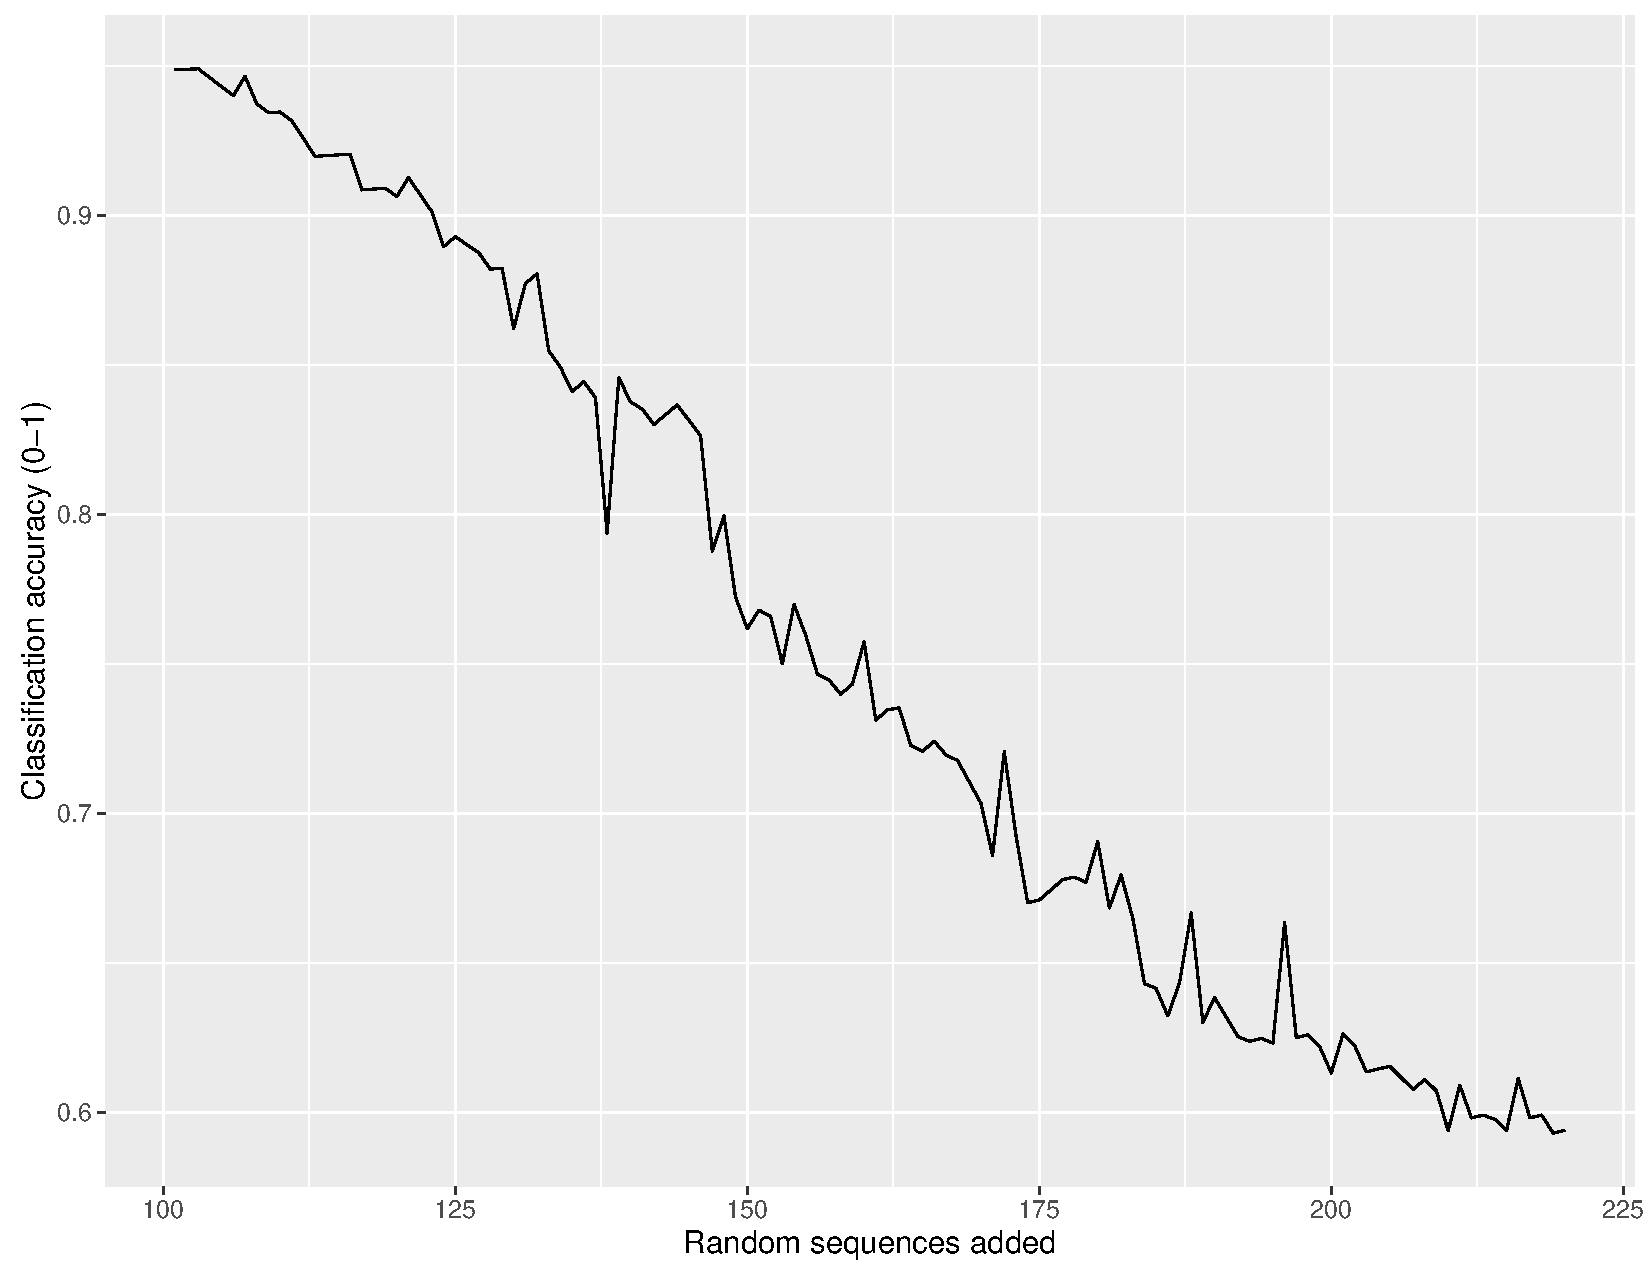
\includegraphics[scale = 0.25]{pics/odseq_accuracy_random_linear}
    \end{minipage}%
    \begin{minipage}{0.5\textwidth}
        \raggedright
        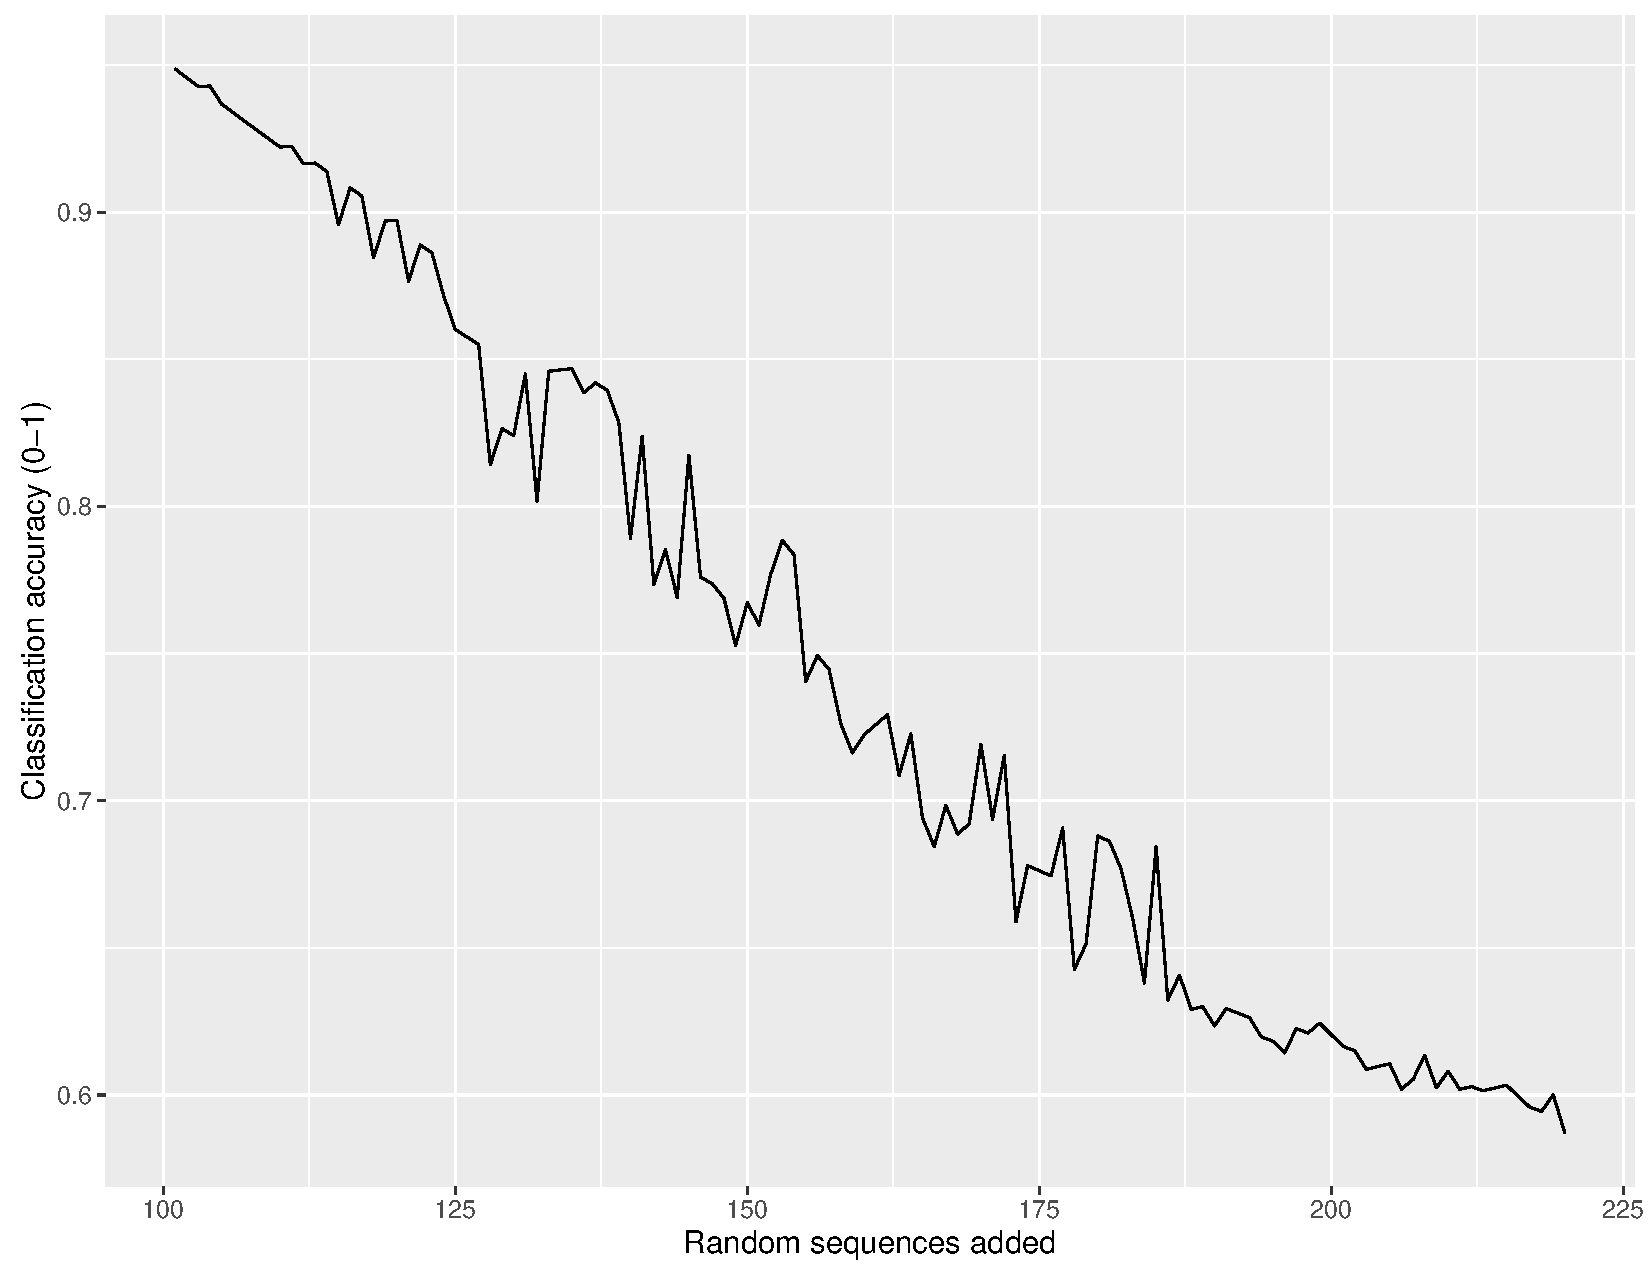
\includegraphics[scale = 0.25]{pics/odseq_accuracy_random_affine}
    \end{minipage}
    \caption{Classification accuracy as the number of random generated sequences inceases. This behaviour is because the mean of the distance bootstrap replicated is shifted to the average of the outliers instead of the non-outliers.} 
\label{fig:odseq_accuracy_random}
\end{figure}

We also considered $250$ sequences, $200$ belonging to the \texttt{PF01500} family and the remaining to the \texttt{PF13885} family. Both families are under the PFAM \texttt{Keratin-assoc} clan, therefore some relationship exists among both families. The \texttt{odseq} algorithm achieved a $0.664$ accuracy (out of $1$) using the affine metric and 1000 boostrap replicates. Again, as we increment the number of sequences belonging to \texttt{PF13885} the mean will slowly shift to the average of this group, decrementing accuracy.

\subsection{\texttt{unaligned-odseq} results}

As we mentioned before, \texttt{unaligned-odseq} performance depends heavily on the choice of kernel used for the computation of the similarity matrix. First of all, we consider again \texttt{PF09274} and 100 random sequences to compare performance against the aligned version of the algorithm and consider several different kernels. Results of accuracy can be seen in table \ref{accuracy_unal}.\\ 

\begin{table}[]
\centering
\caption{Performance for some kernels used in the \texttt{unaligned-odseq} algorithm.}
\label{accuracy_unal}
\begin{tabular}{@{}ll@{}}
\toprule
\textbf{String kernel}                               & \textbf{Accuracy (0-1)} \\ \midrule
Spectrum kernel (k=3)                                & 0.7781                  \\
Spectrum kernel (k =3, linear distance, sigma=20)  & 0.7588                  \\
Spectrum kernel (k=3, gaussian distance, sigma=10) & 0.7814                  \\
Spectrum kernel (k=3, SWD distance)                  & 0.6624                  \\
Gappy Pair kernel (k=3, m=2)                         & 0.6881                  \\
Gappy Pair kernel (k=1, m=3)                         & 0.8264                  \\
Mismatch kernel (k=3, m=1)                           & 0.6334                  \\ \bottomrule
\end{tabular}
\end{table}

In this particular example, most kernels seem to behave similarly, and some parameter tuning may be needed in each specific problem. However, the Spectrum kernel seems to behave very regularly when using different distance weights using $k=3$. Further research may be needed to find a robust kernel that would provide acceptable performance in most of the usual cases. However, we notice quickly that as expected, performance on the unaligned version of the algorithm is not as good compared to its aligned counterpart.\\

We also considered sequences belonging to the same PFAM clam in our experiments (200 from \texttt{PF01500} and  50 from \texttt{PF13885}) as we expect to see performance drops just as in the last case. Surprisingly, \texttt{unaligned-odseq} seems to perform way better than plain \texttt{odseq} when sequences are somewhat related to each other, achieving $0.92$ accuracy using the Gappy Pair kernel and $0.932$ using the Spectrum kernel. This suggests that the unaligned algorithm should be used when one knows of some relationships in the sequences.

\subsection{Mixtures experiments}

In this subsection, we test the last of the algorithms proposed in the paper, that is, the use of Gaussian mixtures for identifying several different alignments to perform. In the same sense as the previous two sections, one can use mixtures for outlier detection as well, if two is chosen as the number of components. For example, measuring accuracy incrementing the number of random sequences with \texttt{PF09274} yields the results visible in figure \ref{fig:mixac}.\\

\begin{figure}
\centering
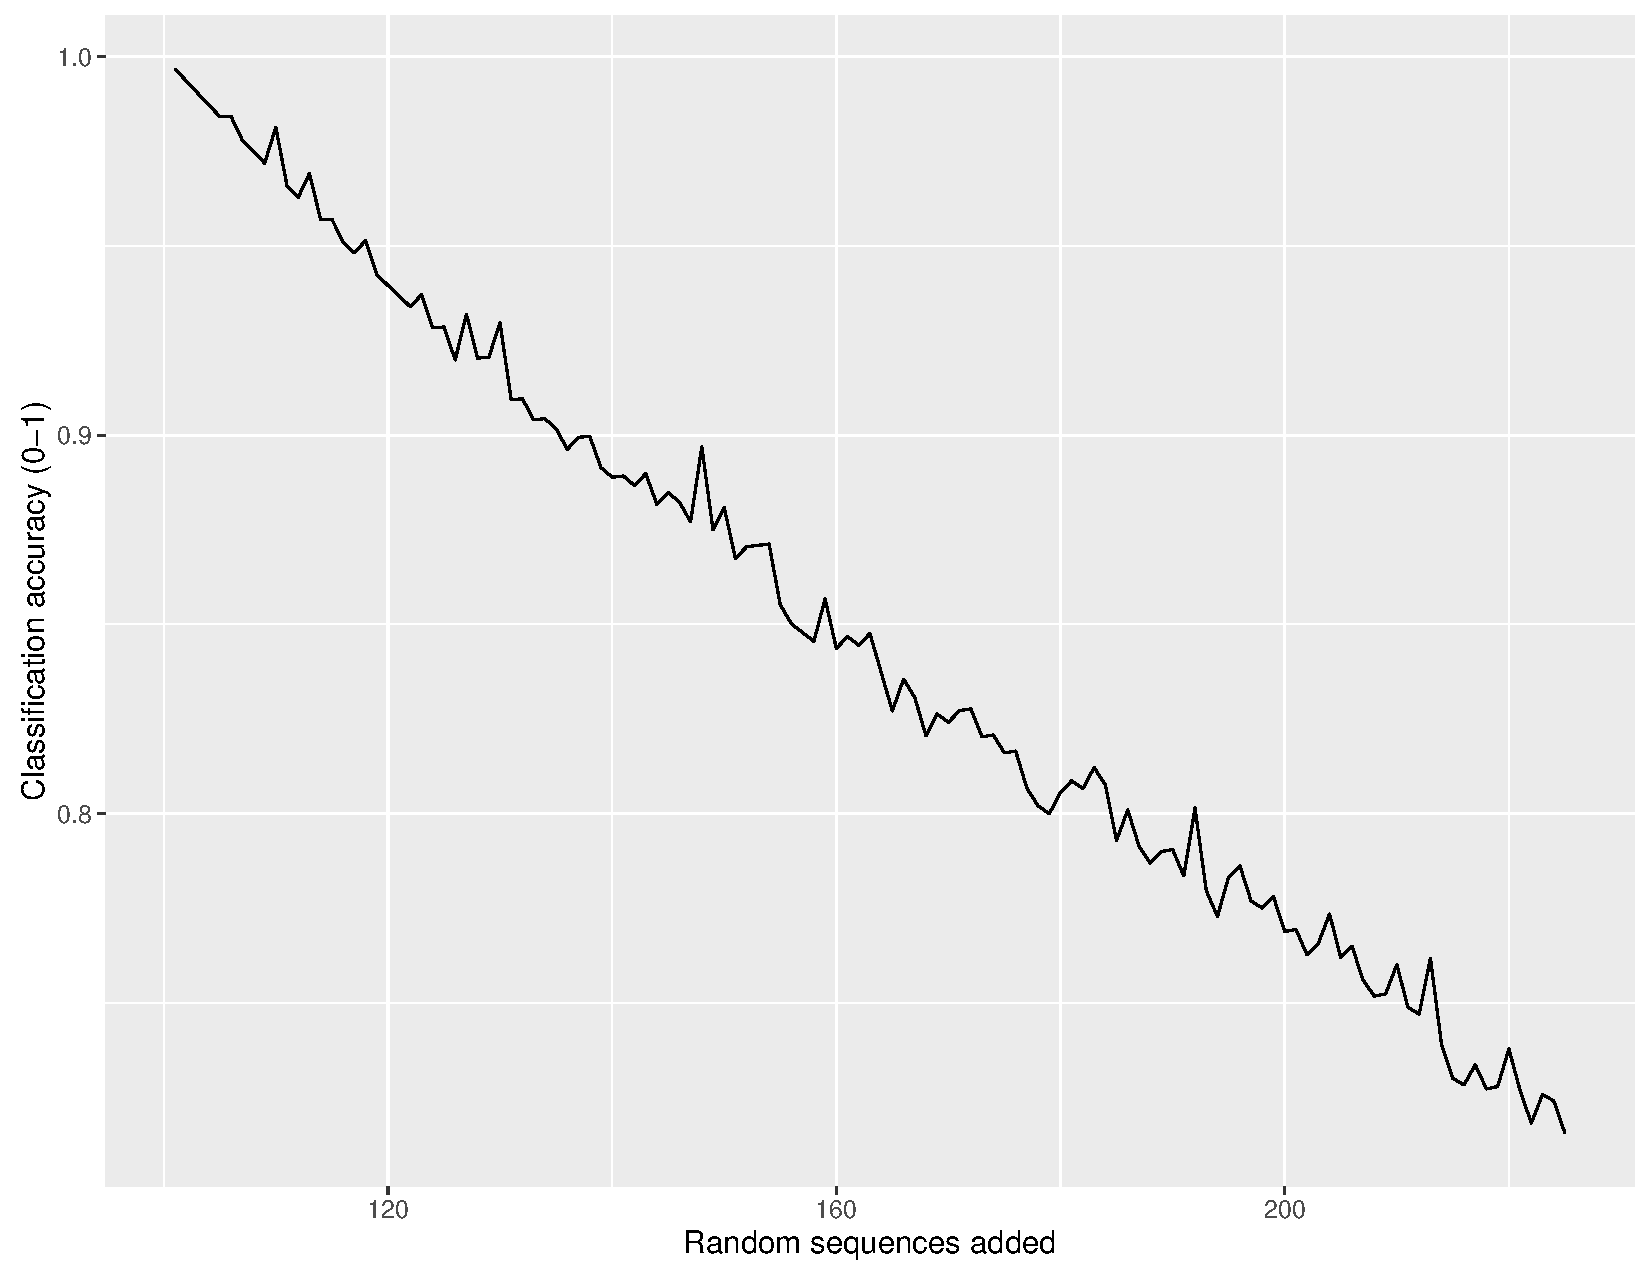
\includegraphics[scale=0.3]{pics/mixac}
\caption{Accuracy (0-1) for outlier detection using the gaussian mixture model with affine metric adding random sequences.}
\label{fig:mixac}
\end{figure}

However, in this case we are more interested in detecting several possible alignments from one big population of sequences. Following the same pattern as in the last experiments, we pick 3 families of sequences (\texttt{PF01500}, \texttt{PF13885} and \texttt{PF05267} belonging to the \texttt{Keratin assoc} clan) with sizes 200 each and measure multiclass classification accuracy. In particular, the mixture model was able to achieve a multiclass accuracy of 0.5034, which, taking into account there are more than 2 groups, it is an acceptable result. A plot of the classification can be seen in figure  \ref{fig:class_mix}.

\begin{figure}
\centering
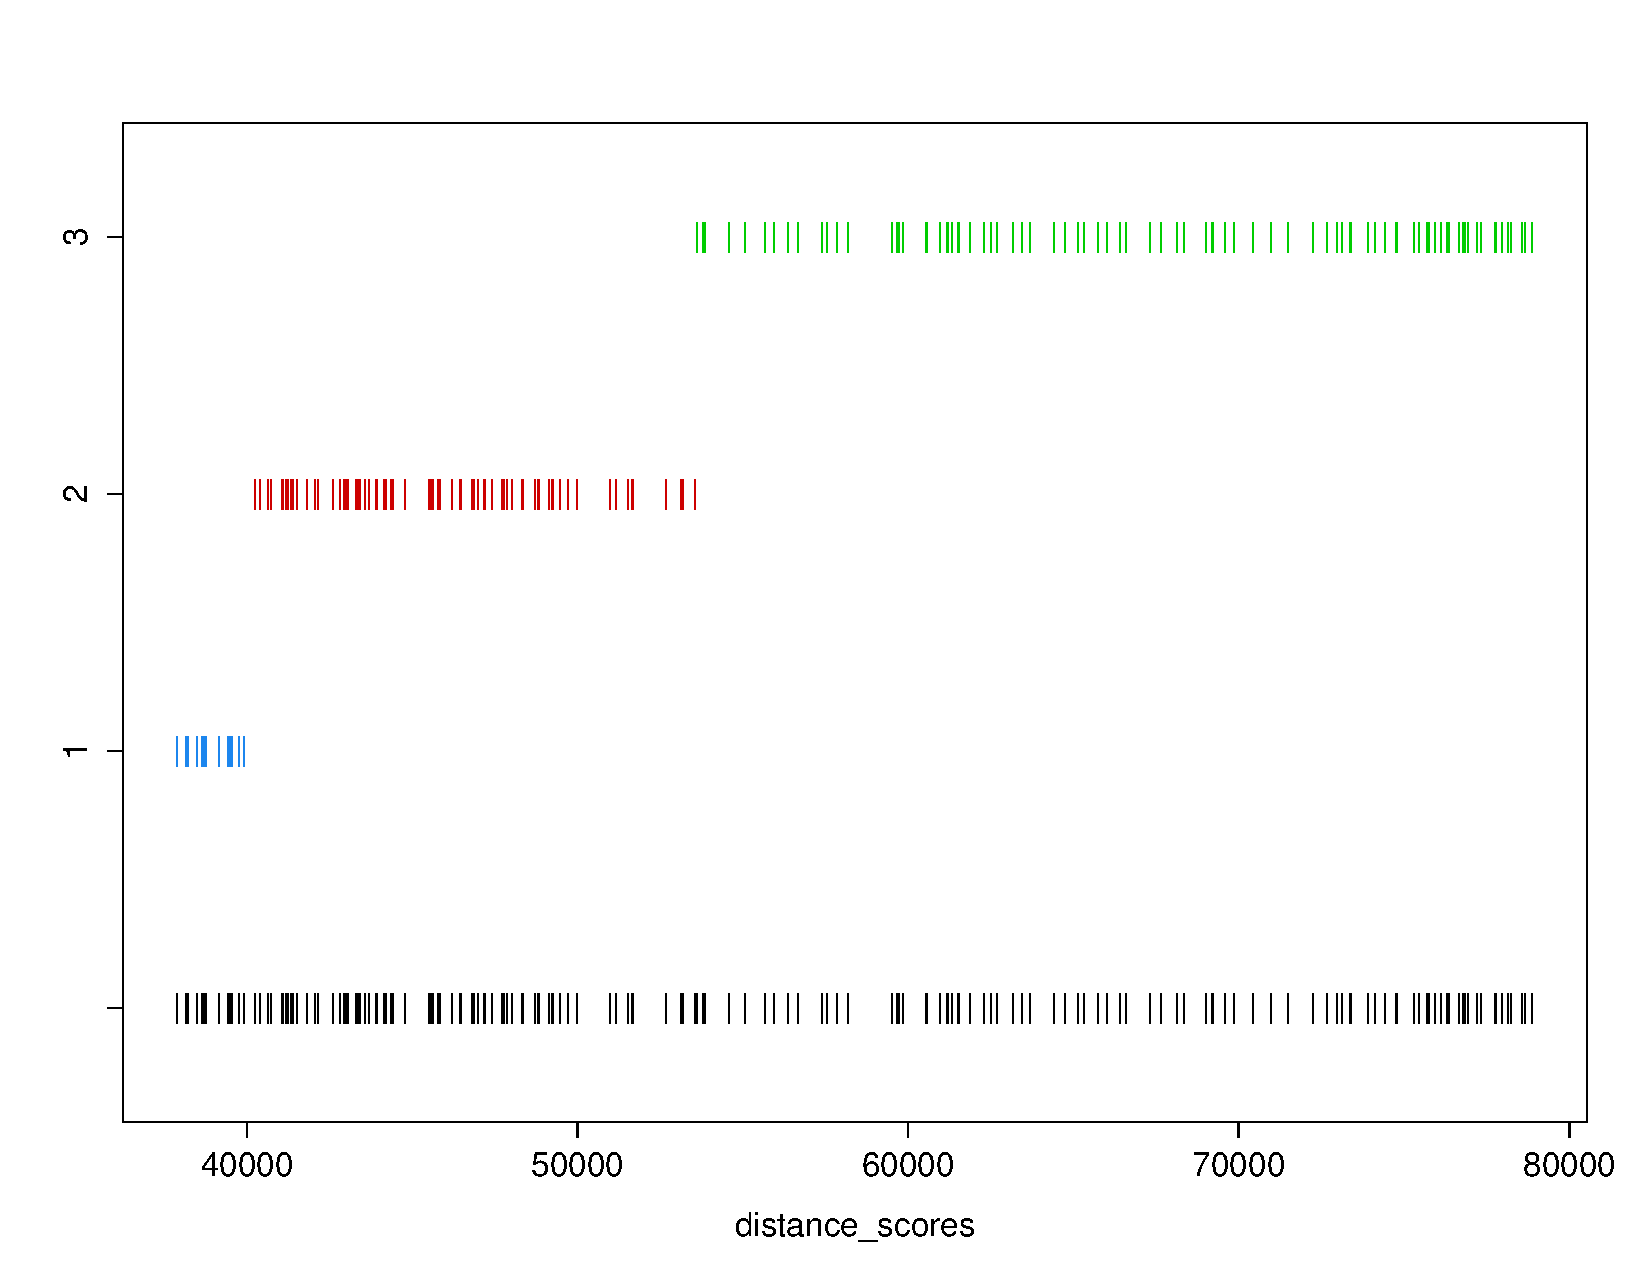
\includegraphics[scale=0.3]{pics/class_mix}
\caption{Classification plot for the mixture model using 3 groups. It can be appreciated that the mixture has trouble distinguishing the elements from the first and second populations in particular, the third one remaining the easiest to discriminate.}
\label{fig:class_mix}
\end{figure}


\section{Conclusion and remarks}

We presented improvements to the \texttt{odseq} algorithm, and presented new variant using kernel functions for its unaligned version. In particular, the aligned counterpart seems to behave best when the groups of the sequences are not very related to each other, while \texttt{unaligned-odseq} performed very well in experiments where sequences belong to the same PFAM clan. In particular, \texttt{odseq} has trouble distinguishing groups when the pattern of the distances is similar among groups. To improve the algorithms' performance using other techniques remains a topic of further research. We also proposed a Gaussian mixture model to distinguish among several alignments with yielded acceptable results in our experiments.

\nocite{*}
\bibliography{bibliography}{}
\bibliographystyle{plain}

\end{document}